% -*- TeX-master: "main"; fill-column: 72 -*-

\section{Introduction and Motivation}

In the context of SBML, hierarchical model composition refers to the
ability to include models as submodels inside other models. The goal is
to support the ability of modelers and software tools to do such things
as (1) decompose larger models into smaller ones, as a way to manage
model complexity; (2) incorporate multiple instances of the same
component model within one or more enclosing models, to avoid literal
duplication of repeated elements; and (3) create libraries of vetted
models, much as is done in software development and other engineering
fields. This document describes a proposal for an SBML Level~3 package
to support hierarchical model composition.  \fig{fig1} illustrates
some of the scenarios targeted by this proposal.

\begin{figure}[b]
  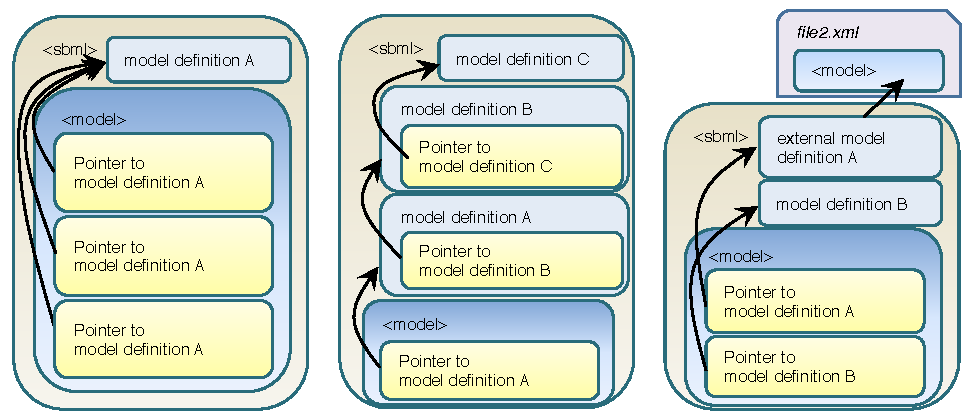
\includegraphics{figs/figure1}
  \caption{Three different examples of model composition scenarios.
    From left to right: (1) a model composed of multiple instances of a
    single, internally-defined submodel definition; (2) a model composed
    of a submodel that is itself composed of submodels; and (3) a model
    composed of submodels, one of which is defined in an external file.}
  \label{fig1}
\end{figure}

SBML Level 3 Core has no direct support for allowing a model to include
other models as submodels. Software tools either have to implement their
own schemes outside of SBML, or (in principle) one could also use
annotations to augment a plain SBML Level~2 model with the necessary
information to allow a software tool to compose a model out of
submodels.  However, such solutions would be proprietary and
tool-specific, and not conducive to interoperability. There is a clear
need for an official SBML language facility for hierarchical model
composition.

The effort to create a hierarchical model composition mechanism in SBML
has a long history, which we summarize in the next section.  It has also
been known by different names.  Originally, it was called
\emph{modularity} because it allows a model to be divided into
structural and conceptual modules. It was renamed \emph{model
  composition} when it became apparent that the name ``modularity'' was
too-easily confused with other notions modularity, particularly
XHTML~1.1~\cite{} modularity (which concerns decomposition into separate
files).  To make clear that the purpose is structural \emph{model}
composition, regardless of whether the components are stored in separate
files, the SBML community adopted the name SBML \emph{Hierarchical Model
  Composition}.

To support a variety of composition scenarios, this package provides for
optional black-box encapsulation by means of defined data communication
interfaces (here called \emph{ports}).  In addition, it also separates
model \emph{definitions} (i.e., blueprints, or templates) from
\emph{instances} of those definitions, it supports optional external
file storage, and it allows recursive model decomposition with arbitrary
submodel nesting.


\section{Background and previous work}
\label{sec:background}

The focus of this section is on discussing prior work on the topic of
model composition in SBML, and how the current specification relates to
that prior work.


\subsection{Proposal corresponding to this specification}


\subsection{Past work on this problem or similar topics}

The SBML community has discussed the need to add model composition
features to SBML since its very beginning, some ten years ago.  In an
internal discussion document titled \emph{Possible extensions to the
  Systems Biology Markup Language}~\cite{} principally authored by Andrew Finney
(and, notably, written even before SBML Level 1 Version 1 was finalized
in March of 2001), the first of the four titular possible extensions is
for ``submodels''. In that document, the main model object can contain a
list of submodels, each of which are model definitions only, and a list
of submodel instantiations, each of which are references to elements in
the submodel list.  Finney's proposal also extends the syntax of SBML
identifiers (the \primtype{SId} data type) to allow entity references
using a dotted notation, in which \texttt{X.y} signifies element
\texttt{y} of submodel instance \texttt{X}; the proposal also defines a
form of linking model elements through ``substitutions''.  In addition,
the proposal also introduces the concept of validation through what it
called the ``expanded'' version of the model (now commonly referred to
as the ``flattened'' form, meaning translation to a plain SBML format
that does not use composition features): if the flat version of the
model is valid, then the model as a whole must also be valid.

In June of 2001, at the Third Workshop on Software Platforms for Systems
Biology, Martin Ginkel and J\"{o}rg Stelling presented their proposal
titled ``XML Notation for Modularity''~\cite{}, complete with an
accompanying proposal document and sample XML file, partially in
response to deficiencies or missing elements they believed existed in
the proposal by Finney.  In their proposal, Ginkel and Stelling present
a ``classic view'' of modularity, where models are packaged as black
boxes with interfaces.  One of their design goals is to support the
substitution of one module for another with the same defined interface,
thereby supporting the simplification or elaboration of models as
needed.  Their proposal emphasizes the reuse of models and with the
possibility of developing libraries of models.

Martin Ginkel presented an expanded version of that proposal~\cite{} at
in the July 2002 Fifth Workshop on Software Platforms for Systems
Biology, in the hope that it could be incorporated into the definition
of SBML Level 2 that was being developed at the time.  This proposal
clarified the need to separate model definitions from model
instantiations, and, further, the need to designate one model per
document as the ``main'' model.

In March of 2003, an independent proposal~\cite{} by Jonathan Webb was
posted to the sbml-discuss mailing list.  This proposal included a
unified, generic approach to making links and references to elements in
submodels using XPath.  Previous proposals used separate mechanisms for
species, parameters, compartments, and reactions.  Webb also raised the
issue of how to successfully resolve conflicting attributes of linked
elements, debated whether formal interfaces were necessary or even
preferable to directly access model elements, discussed type checking
for linkages, and discussed issues with unit incompatibilities.  Around
this time, Martin Ginkel formed the Model Composition Special Interest
Group~\cite{} a group that eventually reached 18 members, including
Jonathan Webb.

Model composition did not make it into SBML Level 2 when that
specification was released in June of 2003, because the changes between
SBML Level 1 and Level 2 were already substantial enough that software
developers at the time expressed a desire to delay the introduction of
composition to a later revision of SBML.  Andrew Finney (now the
co-chair of the Model Composition SIG) presented yet another
proposal~\cite{} in May of 2003, even before SBML Level 2 Version 1 was
finalized, that aimed to add model composition to SBML Level 3.  With
only two years having passed between SBML Level 1 and Level 2, the
feeling at the time was that Level 3 was likely to be released in 2005
or 2006, and the model composition proposal would be ready when it was.
However, Level 2 ended up occupying the SBML community longer than
expected, with four versions of Level 2 produced to adjust features in
response to user feedback and developers' experiences.

In the interim, the desire to develop model composition features for
SBML continued unabated.  Finney revised his 2003 proposal in October
2003~\cite{}; this new version represented an attempt to synthesize the
earlier proposals by Ginkel and Webb, supplemented with his own original
submodel ideas, and was envisioned to exist in parallel with another
proposal by Finney, for arrays and sets of SBML elements (including
submodels)~\cite{}.  Finney attempted to resolve the differences in the
two basic philosophies (essentially, black-box versus white-box
encapsulation) by introducing optional ``ports'' as interfaces between a
submodel and its containing model, as well as including an XPath-based
method to allow referencing model entities.  The intention was that a
modeler who wanted to follow the classic modularity (black-box) approach
could do so, but other modelers could still use models in ways not
envisioned by the original modeler simply by accessing a model's
elements directly via XPath-based references.  In both schemes, elements
in the submodels were replaced by corresponding elements of the
containing model.  Finney's proposal also provided a direct link
facility that allows a containing model to refer directly to submodel
elements without providing placeholder elements in the containing
model.  For example, a containing model could have a reaction that
converts a species in one submodel to a species in a different submodel,
and in the direct-link approach, it would only need to define the
reaction, with the reactant and product being expressed as links
directly to the species defined in the submodels.

After Finney's last effort, activities in the SBML community focused on
updates to SBML Level 2, and since model composition was slated for
Level 3, not much progress was made for several years, apart from Finney
including a summary of his 2003 proposal and of some of the unresolved
issues in a poster~\cite{} at the 2004 Intelligent Systems for Molecular
Biology (ISMB) conference held in Glasgow.

Finally, in June of 2007, unplanned discussions at the Fifth SBML
Hackathon~\cite{} prompted the convening of a workshop specifically to
revitalize the model composition package, and in September of 2007, the
SBML Composition Workshop~\cite{} was held at the University of
Connecticut Health Center, hosted by the Virtual Cell group and
organized by Ion Moraru and Michael Blinov.  This event produced several
artifacts, still available online:

\begin{enumerate}

\item Martin Ginkel provided a list of goals for model
  composition~\cite{}, including use cases, and summarized many of the
  issues discussed in the present document to this point, including the
  notion of definition versus instantiation, linking, referencing
  elements that lack SBML identifiers, and the creation of optional
  interfaces.  It also mentioned the need of allowing parameterization
  of instances (i.e., setting new numerical values that override the
  defaults), and the need to be able to ``delete'' or elide elements out
  of submodels.  (He also provided a summary of ProMoT's model
  composition approach and a summary of other approaches~\cite{}.)

\item Andrew Finney wrote up a list of issues and comments, recorded
  on the meeting wiki page~\cite{}; these included some old issues as
  well as some new ones:

  \begin{itemize}

  \item There should perhaps be a flag for ports to indicate whether a
    given port must be overloaded.

  \item There should be support for N-to-M links, when a set of elements
    in one model are replaced as a group, conceptually, with one or more
    elements from a different model.

  \item The proposal should be generic enough to accommodate future
    updates and other SBML Level 3 packages.

  \end{itemize}
  
  \item Wolfram Liebermeister presented his group's experience with
    SBMLMerge~\cite{}, dealing with the pragmatics of merging multiple
    models.  As far as this proposal goes, he noted that the annotations
    in a composed model need to be considered, particularly since they
    can be crucial to successfully merging models in the first place.

  \item On behalf of Ranjit Randhawa, Cliff Shaffer summarized Ranjit's
    work in the JigCell group on model fusion, aggregation, and
    composition~\cite{}.  Highlights of this presentation and work
    include the following:

    \begin{itemize}

    \item A description of different methods which all need some form of
      model composition, along with the realization that model fusion
      and model composition, though philosophically different, entail
      exactly the same processes and require the same information.

    \item A software application (the JigCell Composition Wizard) that
      can perform conversion between types.  The application can, for
      example, promote a parameter to a species, a concept which had
      been assumed to be impossible and undesirable in previous
      proposals.  

    \item The discovery that merging of SBML models should be done in
      the order Compartments $\rightarrow$ Species  $\rightarrow$
      Function Definitions  $\rightarrow$ Rules  $\rightarrow$ Events
      $\rightarrow$ Units  $\rightarrow$ Reactions  $\rightarrow$
      Parameters.  If done in this order, potential conflicts are
      resolved incrementally along the way.

    \end{itemize}

  \item Nicolas Le~Nov\`{e}re created a proposal for SBML modularity in
    Core~\cite{}.  This is actually unrelated to the efforts described
    above; it is an attempt to modularize a ``normal'' SBML model in the
    sense of divvying up the information into modules or blocks, rather
    than composing a model from different chunks.  It was agreed at the
    workshop that this is a completely separate idea, and while it has
    merits, should be handled separately.

  \item As a collective, the group produced an ``Issues to Address''
    document~\cite{}, with several conclusions:


    \begin{itemize}

    \item It should be possible to ``flatten'' a composed model to
      produce a valid SBML Level 3 Core model, and all questions of
      validity can then be simply applied to the flattened model.  If
      the Core-only version is valid, the composed model is valid.

    \item The model composition proposal should cover both
      designed-ahead-of-time as well as ad-hoc composition. (The latter
      refers to composing models out of components that were not
      originally developed with the use of ports or the expectation of
      being incorporated into other models.)

    \item The approach probably needs a mechanism for deleting SBML
      model elements.  The deletion syntax should be explicit, instead
      of being implied by (e.g.) using a generic replacement construct
      and omitting the target of the replacement.

    \item It should be possible to link any part of a model, not just
      (e.g.) compartments, species and parameters.

    \item The approach should support item ``object
      overloading''~\cite{} and be generally applicable to all SBML
      objects.  However, contrary to what is provided in the JigCell
      Composition Wizard, changing SBML component types is not supported
      in object overloading.

    \item A proposition made during the workshop is that elements in the
      outer model always override elements in the submodels, and perhaps
      that sibling linking be disallowed.  This idea was hotly debated.

    \item Interfaces (ports) are indeed considered helpful, but should
      be optional.  They do not need to be directional as in the
      electrical engineering ``input'' and ``output'' sense---the outer
      element always overrides the inner element, but apart from that,
      biology does not tend to work in the directional way that
      electrical components do.

    \item The ability to refer to or import external files may need a
      mechanism to allow an application to check whether what is being
      imported is the same as it was when the modeler created the
      model.  The mechanism offered in this context was the use of MD5
      hashes.

    \item A model composition approach should probably only allow
      whole-model imports, not importing of individual SBML elements
      such as species or reactions.  The reason is that model components
      are invariably defined within a larger context, and attempting to
      pull a single piece out of a model is unlikely to be safe or
      desirable.

    \item The model composition approach must provide a means to handle
      the conversion of units, so that the units of entities defined in
      a submodel can be made congruent with the entities that refer to
      them in the enclosing model.

    \end{itemize}

\end{enumerate}

During the workshop, the attendees collectively worked on a rough draft
proposal.  Stefan Hoops acted as principal editor.  The proposal for the
SBML package (which was renamed the \emph{Hierarchical Model
  Composition}~\cite{}), was issued a mere one day after the end of the
workshop.  It represented an attempt to summarize the workshop as a
whole, and provide a coherent whole, suitable as a Level 3 package.  It
provided a brief overview of the history and goals of the proposal, as
well as several UML diagrams of the proposed additions.  Stefan
presented~\cite{} the proposal in August of 2008 at the 13th SBML Forum,
and subsequently gave the same presentation again at the 7th SBML
Hackathon in March of 2009 and at the 14th SBML Forum in September of
2009, in a continuing effort to raise interest.

Roughly concurrently, Herbert Sauro, one of the original developers of
SBML, received a grant to develop a modular human-readable model
definition language, and hired Lucian Smith in November of 2007 to work
on the project.  Sauro and Frank Bergmann, then a graduate student with
Herbert, had previously written a proposal~\cite{} for a human-readable
language that provided composition features, and this was the design
document Lucian Smith initially used to create a system that was
eventually called \emph{Antimony}. Through a few iterations, the
design~\cite{} eventually settled on was very similar in concept
(largely by coincidence) to that developed by the group at the 2007
Connecticut workshop: namely, with model definitions placed separately
from their instantiations in other models, and with the ability to link
(or ``synchronize'', in Antiomony terminology) elements of models with
each other.  Because Antimony was designed to be ``quick and dirty'', it
allowed type conversions much like the JigCell Composition Wizard,
whereby a parameter could become a species, compartment, or even
reaction.  Synchronized elements could end up with aspects of both
parent elements in their final definitions: if one element defined a
starting condition and the other how it changed in time, the final
element would have both.  If both elements defined the same aspect (like
a starting condition), the one designated the ``default'' would be used
in the final version.  Smith developed methods to import other Antimony
files and even SBML models, which could then be used as submodels of
other models and exported as flattened SBML.

At the 2010 SBML-BioModels.net Hackathon, in response to popular demand
from people at the workshop, Smith put together a short
presentation~\cite{} about model composition and some of the limitations
he found with the 2007 proposal.  In particular, he proposed the
separation of the replacement concept (where old references to replaced
values are still valid) from the deletion concept (where old references
to replaced values are no longer valid).  Smith wrote a summary of that
discussion, added some more of thoughts, and posted it to
sbml-discuss~\cite{}.  In this posting, he proposed and/or reported
several possible modifications to the Hoops et al. 2007 proposal,
including the following:

\begin{itemize}

\item Separation of \emph{replacement} from \emph{deletion}.

\item Separation of model definitions from instantiations.

\item Elimination of ports, and the use of annotations instead.

\item Annotation of N-to-M replacements, instead of giving them their
  own construct.

\end{itemize}

The message to sbml-discuss was met with limited discussion.  However,
it turns out that several of the issues raised by Smith were brought up
at the 2007 meeting, and had simply been missed in the generation of the
initial (and incomplete) proposal placed on the wiki after the
workshop.  The group had, for example, originally preferred to
differentiate deletions from replacements more strongly than by simply
having an empty list of replacements, and omitted them simply because no
better method could be found.  Similarly, the separation of definitions
from instantiations had been a part of every proposal up until 2007, and
was mentioned in the notes for that meeting.  The decision to merge the
two was a last-minute design decision brought about when the group noted
that if the XInclude construct was used, the separation was not strictly
necessary from a technical standpoint.

Smith joined the SBML team part-time in September of 2010, and was
tasked with going through the old proposals and synthesizing from them a
new version that would work with the final incarnation of SBML Level 3.
That version (the first version of this document) was presented at
COMBINE in October 2010~\cite{}, and further discussed on the
sbml-discuss mailing list.  At HARMONY in April of 2011, consensus was
reached on a way forward for resolving the remaining controversies
surrounding the specification, resulting in the current version of this
document.


\subsection{Genesis of the current proposal}

A candidate Level 3 Version 1 Core specification was not released until
the end of 2009, and it was only in October of 2010 that the final Level
3 Version 1 Core specification was released.  As a consequence of the
lack of a concrete, finalized SBML Level 3 Core specification, all of
the model composition efforts up to this point have been theoretical:
they could not define a precise syntax as long as the underlying SBML
Level 3 syntax was not finalized.  The few SBML-compatible software
tools that \emph{did} implement some form of composition had to do so
using proprietary approaches or extensions to SBML. This has now
changed, thanks to the finalization of SBML Level 3 Version 1 Core, and
the present proposal is an attempt to blend features of previous efforts
into a concrete, Level 3-compatible syntax.

The current proposal was written from scratch, but draws strongly on the
Hoops 2007 and Finney 2003 proposals, as well as, to some degree, every
one of the sources mentioned above.  Some practical decisions are new to
this proposal, sometimes due to additional design constraints resulting
from the final incarnation of SBML Level 3, but all of them draw from a
wealth of history and experimentation by many different people over the
last decade.  Where this proposal differs from the historical consensus,
the reasoning is explained, but for the most part, the proposal follows
the road most traveled, and focuses on being clear, simple, only as
complex as necessary, and applicable to the largest number of
situations.


\subsection{Design goals of the current proposal}

The following are the basic design goals followed in this proposal:

\begin{itemize}

\item \emph{Allow modelers to build models by aggregation, composition,
    or modularly}.  These methods are so similar to one another, and the
  process of creating an SBML Level 3 package is so involved, that we
  believe it is not advantageous to create one SBML package for
  aggregation and composition, and a separate package for modularity.
  Users of the hierarchical model composition package should be able to
  use and create models in the style that is best suited for their
  individual tasks, using any of these mechanisms, and to exchange and
  reuse models from other groups simply and straightforwardly.

\item \emph{Interoperate cleanly with other packages}. The rules of
  composition should be such that they could apply to any SBML element,
  even unanticipated elements not defined in SBML Level 3 Core and
  introduced by some future Level 3 package.

\item \emph{Allow models produced with these constructs to be valid SBML
    if the constructs are ignored}.  As proposed by Nicolas
  Le~Nov\`{e}re and affirmed by the SBML Editors~\cite{}, whenever
  possible, ignoring elements defined in a Level 3 package namespace
  should result in syntactically-correct SBML models that can still be
  interpreted to some degree, even if it cannot produce the intended
  simulation results of the full (i.e., interpreting the package
  constructs) model.  For example, inspection and visualization of the
  Core model should still be possible.

\item \emph{Ignore verbosity of models}. We assume that software will
  deal with the ``nuts and bolts'' of reading and writing SBML.  If
  there are two approaches to designing a mechanism for this
  hierarchical composition package, where one approach is clear but
  verbose and the other approach is concise but complex or unobvious, we
  prefer the clear and verbose approach.  We assume that software tools
  can abstract away the verbosity for the user.  (However, tempering
  this goal is the next point.)

\item \emph{Avoid over-complicating the specification}. Apart from the
  base constructs defined by the proposal, any new element or attribute
  being introduced should have a clear use case that cannot be achieved
  in any other way.  

\item \emph{Allow modular access to files outside the modeler's
    control}.  In order to encourage direct model referencing (such as
  to models hosted online on sites such as BioModels.net~\cite{}),
  whenever possible, we will require referenced submodels only to be
  SBML Level~3 Core, and not require that they include constructs from
  this proposal.

\item \emph{Incorporate most, if not all, of the desirable features of
    past proposals}. The names may change, but the aims of past efforts
  at SBML model composition should still be achievable with the present
  proposal.

\end{itemize}


\section{Proposed syntax and semantics}
